\documentclass{article}
\usepackage{multicol}
\usepackage{graphicx}% Include figure files
\usepackage{dcolumn}% Align table columns on decimal point
\usepackage{bm}% bold math
\usepackage{hyperref}% add hypertext capabilities
\usepackage{booktabs}
\usepackage{listings}
\usepackage{mathtools}
\usepackage{amsmath}
\renewcommand{\abstractname}{\vspace{-\baselineskip}}
\bibliographystyle{plain}
\usepackage[utf8]{inputenc}
\usepackage{verbatim} %for å inkludere filer med tegn LaTeX ikke liker
\usepackage{mathpazo}
\usepackage{float}
\usepackage{algpseudocode}
\newcommand\numberthis{\addtocounter{equation}{1}\tag{\theequation}}
\usepackage[left=20mm,right=20mm,top=33.95mm,bottom=33.95mm]{geometry} 
% Justerer bredden på columns.
\setlength{\columnsep}{1cm}

\begin{document}

\title{Project 3}
\author{Sebastian Amundsen, Marcus Berget and Andreas Wetzel}

\maketitle

\begin{abstract}

\end{abstract}

\begin{multicols}{2}

\section{Introduction}

Though simulating a solar system is interesting and fun enough on it's own, it is naturally also quite useful for the study of astrodynamics. In addition, being able to simulate a solar system provides a good set of tools applicable to many other scientific areas. These tools include having a good understanding of different numerical integration methods, and being able to write a structured and fast code. In this project we wish to explore a model of our own solar system, beginning with simulating the simple two-body system including the Earth and the Sun. We will use this system to compare two different methods of numerical integration, the forward Euler method and the velocity Verlet method. This simple system also makes a good testing ground for exploring whether our model is consistent with known physical laws such as energy conservation and Kepler's laws of planetary motion. We will also test the stability of the velocity Verlet method by including Jupiter and playing around with it's mass. From there we will include the rest of the planets in our solar system, and blah blah blag general relativity. 

\section{Theory}
\subsection{Forward Euler}
The forward Euler method is an algorithm to estimate the solution of a differential equation. The Forward Euler method  finds the next positions $\mathbf{r}_{i+1}$ by using the position we are at $\mathbf{r}_{n}$, a small time step $dt$ and the derivative of its position. The forward Euler algorithm updates the position before the velocity, hence the energy is not confirmed. 
The forward Euler algorithm will look like:
\begin{align*}
    \mathbf{r}_{n+1}&=\mathbf{r}_n+\mathbf{v}_ndt\\
    \mathbf{v}_{n+1}&=\mathbf{v}_n+\mathbf{a}_ndt\\
    t_{n+1}&=t_n + dt
\end{align*}
The number of FLOPS in the Forward Euler method is 4 for each time step, when we look at the addition and multiplication of this algorithm. The number of total FLOPS is $4N$, since we are looping over a time period N. It is also important to notice that the forward Euler method does not conserve energy. This is due to the position being updated before the velocity.  \\
For more details see Appendix B.
\\
\subsection{Verlet integration}
The Velocity Verlet method is based on the kinematic equations for a moving object, which in our case is a planets orbit around the sun. For the Velocity Verlet algorithm will the velocity be updated before the position, this leads to conservation of energy.\\   
The general algorithm for the Velocity Verlet:
\begin{align*}
    \mathbf{r}_{n+1}&=\mathbf{r}_n+\mathbf{v}_ndt+\frac{\mathbf{a}_n}{2}dt^2\\
    \mathbf{v}_{n+1}&=\mathbf{v}_n+\frac{\mathbf{a}_{n+1}-\mathbf{a}_n}{2}dt
\end{align*}
NUMBER OF FLOPS\\
For more details see Appendix B.

\section{Method}


\subsection{Program flow}

We will here discuss the program flow of the code we have used to model the solar system. All code can be found at the GitHub repository \\
\url{https://github.com/Sebamun/FYS3150_Projekter/tree/Sebastian/Project3}  \\ The code is mostly based on two classes, a planet class and a solver class. Initializing the planet class creates an instance which contains all the relevant information about a celestial object. When the desired celestial objects are initialized, they can then be added to an instance of the solver class. The solver class contains many different functions, mostly aimed toward aiding the velocity Verlet or Euler function. These two functions are based on using their respective algorithms to print out the relevant information of each time step to output-files. The output files can then be read by python-programs which analyze/plot the data.

\subsection{Comparison of the algorithms}
The timing and counting of number of FLOPS of the algorithms is done by writing two separate programs with the sole purpose of doing only this. Comparing the stability of the algorithms is done by plotting the earth-sun system for different time-steps, with the Sun as the center of mass. For the case of a circular orbit we expect that both the potential and kinetic energies are constant and conserved. This is naturally also something we check that the algorithms uphold. 

\subsection{Earth-Sun system}
We have used the Earth-Sun system to compare the two algorithms, but we will now proceed by ditching the forward Euler method, using only the velocity Verlet method instead. Kepler's second law of planetary motion states that the imaginary line joining a planet and the sons sweeps equal areas of space during equal time intervals as the planet orbits. As shown in the appendix, this is equivalent to conservation of angular momentum. [noe mer om dette]. 

\subsection{Many-body system}

Before we include all the planets of the solar system, we start by including only Jupiter. But instead of using our own manufactured initial conditions, we extract the initial conditions from the NASA website \url{https://ssd.jpl.nasa.gov/horizons.cgi#top}. We write the initial conditions to a text file, before we convert the velocities to $\text{AU/Y}$. We also have to take into account, that the velocities extracted from NASA is relative to the center of mass. We therefore have to subtract the velocity of the center of mass to all the velocities. The velocity of the center of mass of the system is found by 
\begin{align}
v_{cm} = \frac{\sum v_i m_i}{M}
\end{align}
where $M$ is the total mass of all the objects in the system, and $v_i$ and $m_i$ are the respective velocities and masses of the objects. 

\subsection{Perihelion precession of mercury}

Just like all the other planets in orbit around the sun, mercury's orbit has an perihelion precession. However, unlike the other planets, mercury's precession can't be explained only by the gravitional tug from other solar bodies. Mercury's precession deviates from the predicted value by 43 arcseconds per century. The deviation can be explained by general relativity by adding a correction to the Newtonian gravitational force, so that the force becomes
\begin{equation}
\mathbf{F}=-G\frac{M_{\odot}M_{Mercury}}{r^2}\Bigg[1+\Bigg(\frac{3l^2}{r^2c^2}\bigg)\bigg]\frac{\mathbf{r}}{r} \label{eq:relcor}
\end{equation}
where $M_\odot\ $ is the mass of the Sun, $M_{Mercury}$ is the mass of Mercury, $r$ is the distance between Mercury and the Sun, $l = |\vec{r} \times \vec{v}|$ is the magnitude of Mercury’s orbital angular momentum per unit mass, and $c$ is the speed of light in vacuum. We want to see if our code produces the same observations, so we start by setting the simulation time to 100 years. Since the we only want to observe the change in precession due to the correction in the gravitational force, we only simulate the Sun and Mercury. Since 43 arc seconds is a very small change in precession, we use as many integration points as possible. To avoid creating too large text files with information about every timestep, we set up the code such that if we use more than $10^7$ integration points, the code only prints out the final position, and velocity to the text file. We then use those positions and velocities as initial conditions for an additional run where the simulation time is about 0.3 years (a little more than a full orbit of mercury around the sun). We then find which time step the minimum distance between the Sun and Mercury took place. We then use this time step to find how much the y-value of the perihelion position has changed. Finally, we can use this value to find the perihelion precession using
\begin{equation}
\tan(\theta_P) = \frac{y_P}{x_P}
\end{equation}

\section{Results}
\subsection{The Earth-Sun system}
From Keeplers third law we have
\begin{align}
    P^2&=\frac{4\pi^2}{GM_\odot}a^3\\
    GM_\odot&=4\pi^2\frac{AU^3}{yr^2}
\end{align}
\subsection{Conservation of angular momentum}
If we substitute equation 15 into equation 14 
\begin{align}
    \frac{dA}{dt}=\frac{1}{2}\frac{L}{m}
\end{align}
Sine $\frac{dA}{dt}$=constant and the mass m is constant means that the angular momentum also is constant and therefore also conserved.  
\\
\subsection{Escape velocity}
In the figure below we can see the behavior for the Sun-Earth system with different initial velocities. 
\begin{figure}[H]
	\centering
	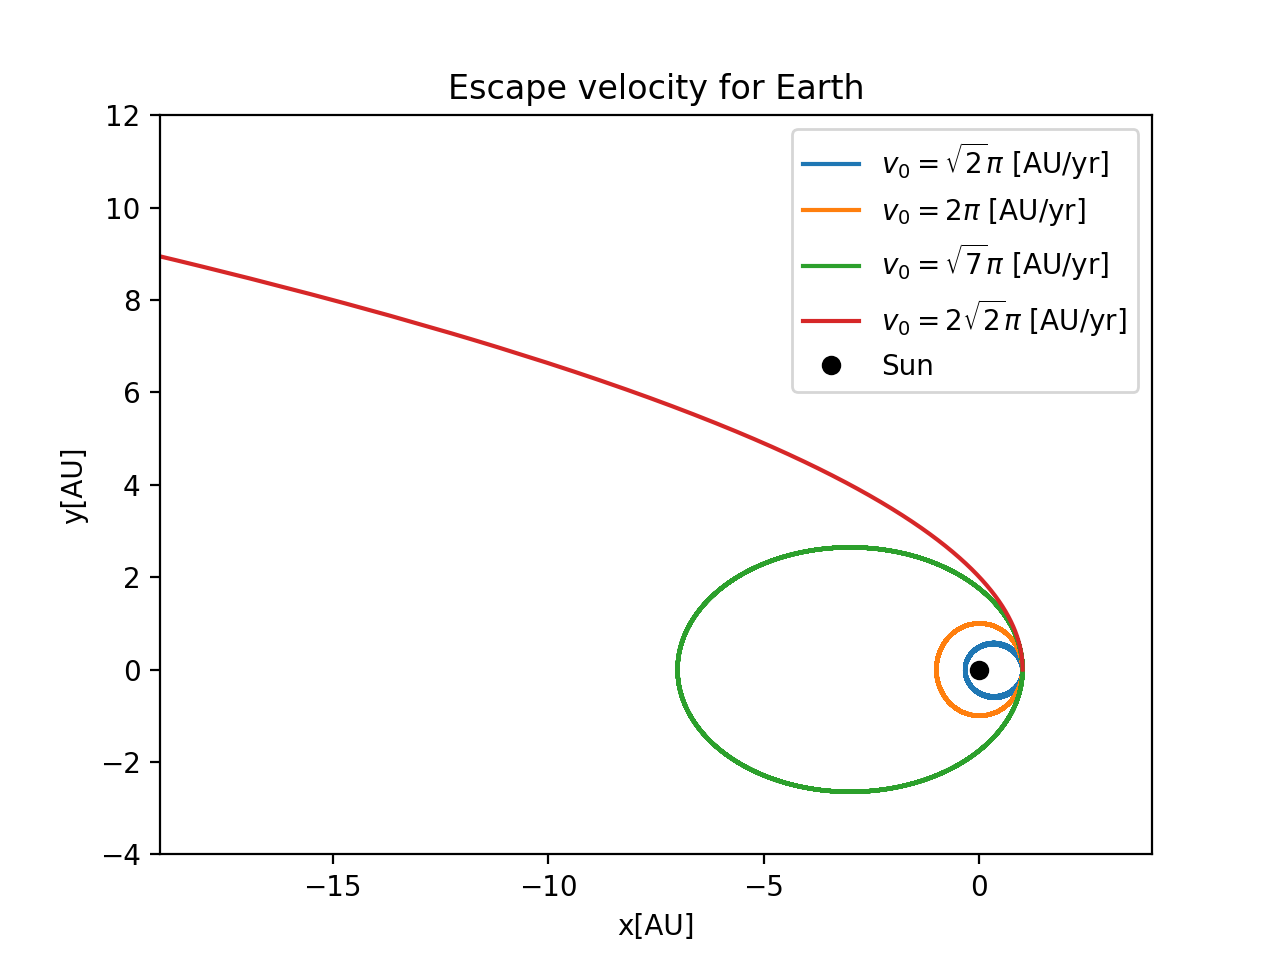
\includegraphics[width=\linewidth]{esc_vel_plot.png}
	\caption{Escape velocity for the Sun-Earth system for different initial velocity}
	\label{fig:1bplot}
\end{figure}
\section{Discussion}
\subsection{Testing forms of the force}
When we let $\beta$ varies between $[2,3]$ we get different results depending on the initial values for position and velocity. If we for example set the distance between the sun and earth $|\mathbf{r}|>AU$ larger then 1 AU, will the gravitational force decrease when we increase $\beta$, and the orbit will get more and more elliptical. \\
If we say that the distance $|\mathbf{r}|<AU$, is larger then 1 AU, the Earth will move towards the sun since the gravitational force will increase when we increase $\beta$.    
\subsection{Escape velocity}
If we increase the initial velocity we see that the orbit of the earth changes from circular orbit to an elliptical orbit, and when the elliptical orbit increase will the position between the two object increase. Hence, will the force of gravity decrease. And when the initial velocity to the planet make it to the escape velocity it will be tear loose from the gravitational field.\\
It is also important to add that we say the center of mass does not move, which means that the center of mass will be constant and it will be very close to the Sun.  

\end{multicols}

\clearpage

\appendix \section{Appendix A} % Her kommer appendix.
\subsection{The Earth-Sun system}
We assume that the earths orbit around the sun is circular. Circular motion and Newtons gravitational force gives us:
\begin{equation}
    F_G=G\frac{M_EM_{\odot}}{r^2}=\frac{M_Ev^2}{r}
    \label{eq:G}
\end{equation}
Where G is the gravitational constant, $M_\odot$ is the mass of the sun, $M_E$ is the mass of the earth, $r$ is the distance between the earth and the sun, and $v$ is the velocity of the moving object (earth). 

We want to show that the velocity $v$ can be written as:

\begin{align}
    v^2r=GM_{\odot}=4\pi^2\frac{AU^3}{yr^2}
    \label{eq:vr}
\end{align}

We can use the centripetal force to rewrite equation \ref{eq:G}, since we are assuming circular orbits:

\begin{align*}
    M_E\omega^2r=G\frac{M_EM_{\odot}}{r^2}
\end{align*}

Where $\omega^2$ is the angular velocity of the earth. Which is given by $\omega^2=2\pi / P$: 

\begin{align*}
    M_E\bigg(\frac{2\pi}{P}\bigg)^2r=G\frac{M_EM_{\odot}}{r^2}\\
\end{align*}

Where $P=1$ year is the period of earth's orbit around the sun.
Now we can use Kepler's third law, which states that the square of an orbital period $P^2$ equals the semi-major axis as it orbits the sun cubed $a^3$. This gives us:

\begin{align}
    P^2=\frac{4\pi^2}{GM_\odot}a^3
\end{align}

Where the circular radius $r$ is substituted with the semi-major axis $a$. In our case $a = 1AU$.  

\subsection{Conservation of angular momentum}

\begin{figure}[H]
	\centering
	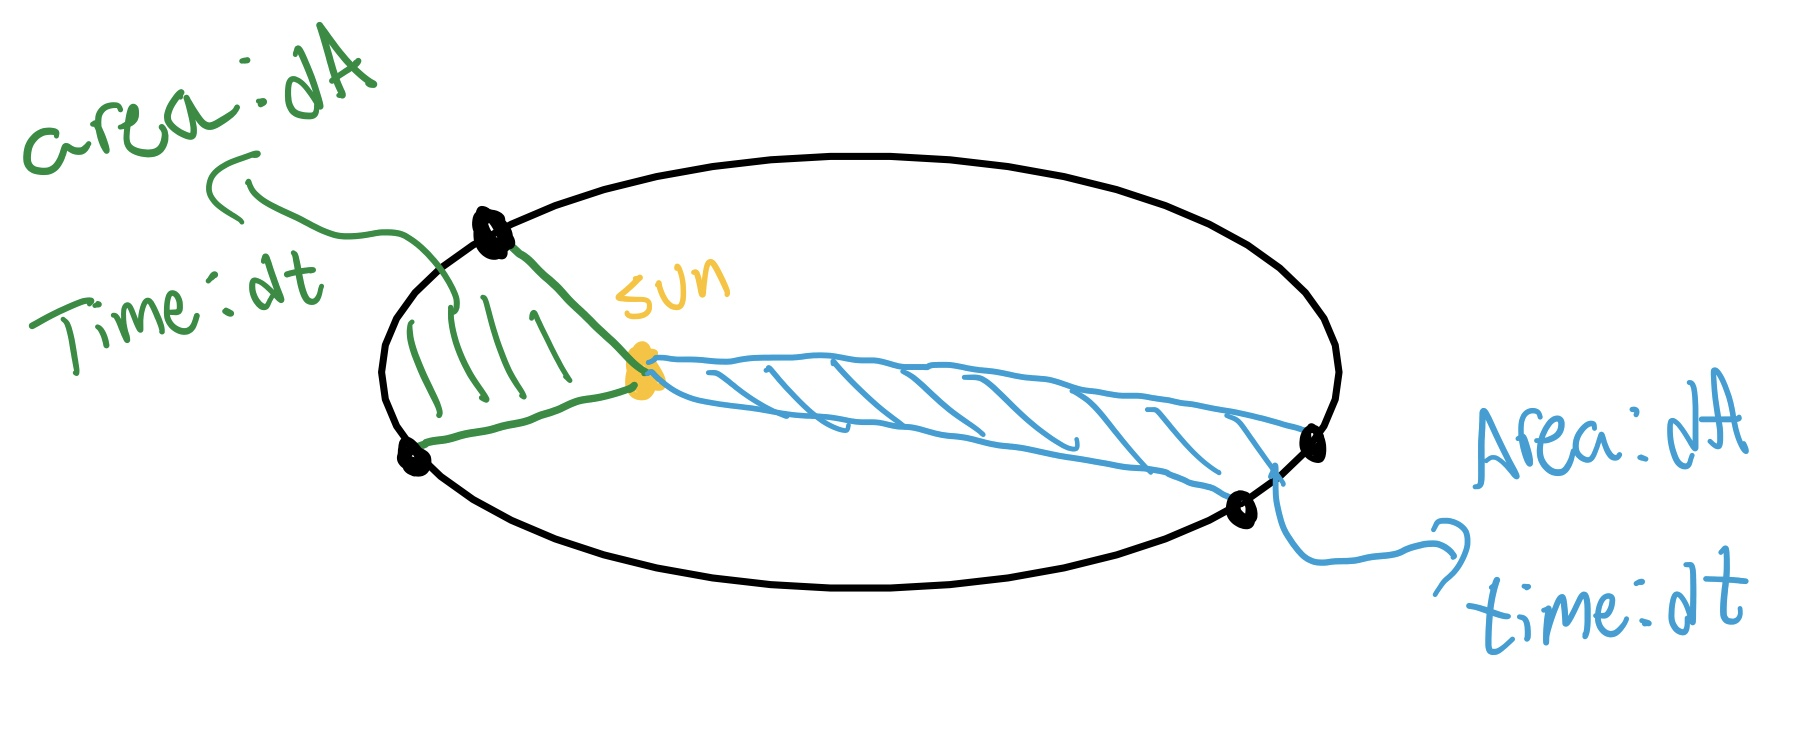
\includegraphics[width=80mm]{K2L.jpg}
	\caption{The area $dA$ is the same for the two time intervals.}
	\label{fig:Kep}
\end{figure}

The definition of Keplers law is that the area $A$, which is formed from a connecting line between a planet and the sun is always the same for a given time interval. This is illustrated in Figure \ref{fig:Kep}.









We have that the angular momentum is 

The best way to show that the angular momentum is conserved by using Keplers second law is to make a drawing:

\begin{figure}[H]
	\centering
	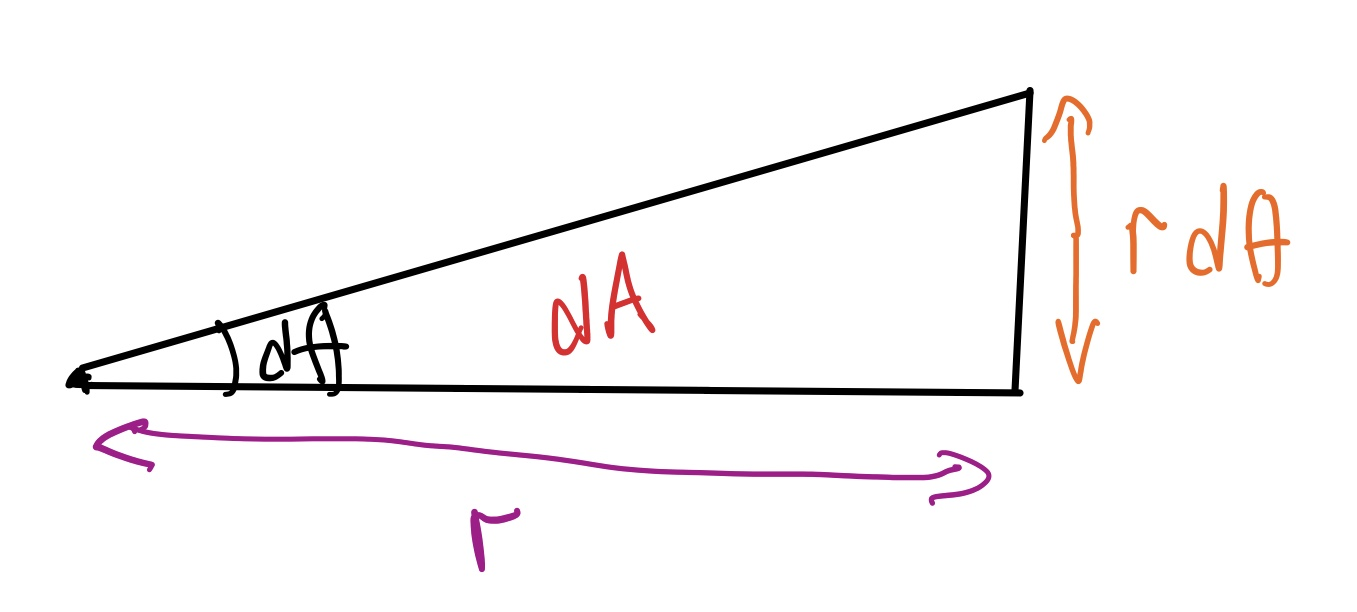
\includegraphics[width=80mm]{sketch.jpg}
	\caption{This square is the infinitesimal area dA that the planet has moved by a infinitesimal time interval dt}
	\label{fig:1bplot}
\end{figure}


Figure 3 shows us that the area is:

\begin{equation}
    dA=\frac{1}{2}r^2d\theta
\label{eq:dA}
\end{equation}

We now want to find an infinitesimal area where the planet has moved around the sun, over an infinitesimal time step, where we use equation 12.

\begin{align}
    \frac{dA}{dt}&=\frac{1}2{r^2}\frac{d\theta}{dt}\\
    &=\frac{1}{2}rv_\theta
\end{align}
And the definition of angular momentum is given as
\begin{align}
    L=mrv_\theta
\end{align}
With equation 14 and 15 we can show that the angular momentum is conserved.
\subsection{Testing forms of the force}
Until now we have looked at the movement for the planet with the gravitational force with the square of r. We will now try to change the gravitational force where the power of r is in the range $\beta \in [2,3]$ The gravitational force is then given as
\begin{align}
    \mathbf{F}_G=-\frac{GM_{\odot}M_{planet}}{r^{\beta}}\frac{\mathbf{r}}{r}
\end{align}
\subsection{Escape velocity}
We will now look at a planet which begins at a distance 1 AU from the sun, 
and see how fast the initial velocity must be for the planet to be able to escape the sun. We find the analytical solution to compare it to our numerical solution. \\
The analytical expression is given as 
\begin{align}
    \mid{\mathbf{V}_{esc}}\mid=\sqrt{\frac{2GM_{\odot}}{r}}
\end{align}
By plugging equation 2 into 16, and use that our initial position of the planet is $r=AU$ we get
\begin{align}
\mid{\mathbf{V}_{esc}^2}\mid&=\frac{2\cdot 4\pi^2AU^3}{yr^2}\cdot\frac{1}{r}\\
&=\frac{2\cdot 4\pi^2AU^3}{yr^2}\cdot\frac{1}{AU}\\
\mid{\mathbf{V}_{esc}}\mid&=2\sqrt{2}\pi\cdot\frac{AU}{yr}
\end{align}
\subsection{Perihelion precision}
LES GJENNOM DETTE MARCUS\\
The definition of perihelion precision is that the perihelion point of an objects, in our case Mercury, changes its position because of 
the gravitational field deflection from light. RIKTIG? The perihelion point for Mercury changes with $43''$ arcseconds for each century. \\
\\
Mercury's orbit has a small prescision for each century. This comes from that Mercury is the nearest planet to the sun, and therefore its acceleration and velocity will be large, which means that the space time will wrap    and we have to obey the rules of General Relativity. Hrnce, we rewrite the expression for Newtons gravitational force to a relativistic gravitational force.
\begin{align}
    \mathbf{F}=-G\frac{M_{\odot}M_{Mercury}}{r^2}\Bigg[1+\Bigg(\frac{3l^2}{r^2c^2}\bigg)\bigg]\frac{\mathbf{r}}{r}
\end{align}

\section{Appendix B} % Her kommer appendix.
\subsection{Forward Euler}
The forward Euler method is an algorithm to estimate the solution of a differential equation. The Forward Euler method  finds the next positions $\mathbf{r}_{i+1}$ by using the position we are at $\mathbf{r}_{n}$, a small time step $dt$ and the derivative of its position. Which can be expressed as:

\begin{equation}
\mathbf{r}_{n+1}=\mathbf{r}_n + \mathbf{r}_n'\cdot dt
\label{eq:yn1}
\end{equation}

Where $\mathbf{r}_n'$ is the derived of the current position. This algorithm is an abbreviated version of a Taylor expansion, where we only expand the series one step at a time. By doing this we will get a local truncation error, which causes an error for each step we take:

\begin{equation}
\begin{split}
&\mathbf{r}(t_n+dt)=\mathbf{r}_{n+1}\\
=&\mathbf{r}(t_n)+dt\bigg(\mathbf{r}'(t_n) + \frac{\mathbf{r}''(t_n)}{2!}dt + ... + \frac{\mathbf{r}^p(t_n)}{p!}dt^{p-1}\bigg) \\
&+ O(dt^{p+1})
\end{split}
\label{eq:ytndt}
\end{equation} 

Where $O(dt^2)$ is the local truncation error. Since the Forward Euler method is a first-order method, the local truncation error will be proportional to the square of the step size.

In our case $\mathbf{r}(t_n) \rightarrow \mathbf{r}_n$ is the position, $\mathbf{r}'(t_n)=\mathbf{v}(t_n) \rightarrow \mathbf{r}'_n=\mathbf{v}_n$ is the velocity and $\mathbf{r}''(t_n)=\mathbf{a}(t_n,r_n) \rightarrow \mathbf{v}_n'=\mathbf{a}_n$ is the acceleration. The update of our position and velocity with a  time step is then given as  
\begin{align*}
    \mathbf{r}(t_{n+1})&=\mathbf{r}(t_n) + \mathbf{v}(t_n)dt + O(dt^2)\\
    \mathbf{r}_{n+1}&=r_{n} + v_{n}dt + O(dt^2)\\
    \mathbf{v}(t_{n+1})&=\mathbf{v}(t_n)+\mathbf{a}_ndt + O(dt^2)\\
    \mathbf{v}_{n+1}&=\mathbf{v}_n +\mathbf{a}_n dt + O(dt^2)
\end{align*}
Hence, the forward Euler algorithm will look like:
\begin{align*}
    \mathbf{r}_{n+1}&=\mathbf{r}_n+\mathbf{v}_ndt\\
    \mathbf{v}_{n+1}&=\mathbf{v}_n+\mathbf{a}_ndt\\
    t_{n+1}&=t_n + dt
\end{align*}
\\
Pseudocode:

\begin{verbatim}
  v[0] = v0   # Boundary conditions
  r[0] = r0   # Boundary conditions

  for (n = 2; n < N-1; n++) {
        V[n+1] = v[n] + a[n] * dt;
        r[n+1] = r[n] + v[n] * dt;
        t[n+1] = t[n] + dt;
        
  }

\end{verbatim}

\subsection{Velocity Verlet method}
The Velocity Verlet method is based on the kinematic equations for a moving object, which in our case is a planets orbit around the sun. If we want to find the next time step for the velocity and position we do an approximation and use a Taylor-expansion:    

\begin{align*}
\mathbf{r}(t\pm dt)&=\mathbf{r}(t)\pm \mathbf{r}'(t)dt + \frac{\mathbf{r}''(t)}{2}dt\\ + O(dt^3)
\end{align*}

This gives us the position and velocity:

\begin{align}
    \mathbf{r}_{n+1}&=\mathbf{r_n}+\mathbf{v}_n dt + \frac{\mathbf{a}_n}{2}dt^2+O(dt^3)
    \label{eq:r_n+1}
    \end{align}
    \begin{align}
    \mathbf{v}_{n+1}&=\mathbf{v}_n+\mathbf{a}_ndt+\frac{\mathbf{v}''_n}{2}dt^2 + O(dt^3)
     \label{eq:v_n+1}
\end{align}

We need to define $\mathbf{v}''_n$. We do this by by defining the next step in acceleration $\mathbf{a}_{n+1}$:

\begin{align*}
    \mathbf{a}_{n+1}=\mathbf{v}'_{n+1}=\mathbf{v}'_n+\mathbf{v}''_ndt + ...
\end{align*}

We can rewrite this as:

\begin{align}
        \mathbf{v}''_n=\frac{\mathbf{v}'_{n+1}-\mathbf{v}_n'}{dt}
    =\frac{\mathbf{a}_{n+1}-\mathbf{a}_n}{dt}
    \label{eq:v_n}
\end{align}

By inserting equation \ref{eq:v_n} into equation \ref{eq:v_n+1} we get the general algorithm for the Velocity Verlet:

\begin{align*}
    \mathbf{r}_{n+1}&=\mathbf{r}_n+\mathbf{v}_ndt+\frac{\mathbf{a}_n}{2}dt^2+O(dt^2)\\
    \mathbf{v}_{n+1}&=\mathbf{v}_n+\frac{\mathbf{a}_{n+1}-\mathbf{a}_n}{2}dt+O(dt^3)
\end{align*}
NUMBER OF FLOPS
\\
Pseudocode:

\begin{verbatim}
  v[0] = v0;   # Boundary conditions
  r[0] = r0;   # Boundary conditions

  for (i = 2; i < n-1; i++) {
      v[n+1] = v[n] + (a[n+1]-a[n]) * dt / 2
      r[n+1] = r[n] + v[n] * dt + a[n] * pow(dt,2) / 2;
  }

\end{verbatim}

\section{Calculations} 

\bibliography{References} % Kilder.
\begin{thebibliography}{9}
\bibitem{94}
	Skriv inn kilde her.
\end{thebibliography}

\end{document}
